\section{Project description}

% \subsection{TEMP: notes to self}

% Outline:

% \begin{itemize}
%  \item Rydberg atom systems are studied in much detail in the last 10 years
%  \item The basic behaviour is well understood, now moving on to ensamble effects
%  \item They are very useful for quantum computing and quantum simulation
%  \item Other system: ion traps are very well advanced and atomic level structure is the same as the atomic Rydberg systems + charge
%  \item Rydberg ions have much richer interactions than the atoms that can be leveraged for good
%  \item The full toolset of ion traps is already available: long storage time, efficient cooling and manipulation
%  \item Proposal exist but not experiments
%  \item Limitations (dephasing time, Rydberg lifetime, scattered light, ground state coherence times)
% \end{itemize}

% Pictures to include:

% \begin{itemize}
%  \item Rydberg ions in trapping potential (length scales, composite system)
%  \item Interaction strength (atom, ion, Rydberg, + add Rydberg ion from the other paper)
% \end{itemize}


% Some more notes from \href{http://sciencecareers.sciencemag.org/career_development/previous_issues/articles/1820/writing_a_research_plan}{here}:
% \begin{itemize}
%  \item Specific
%  \item Short and focus on the major themes
%  \item Solid, realistic plan
%  \item Include redundant aproaches
%  \item 12pt, 1.5 spaced text, 3-5 pages
%  \item include summary
%  \item choose graphics well
%  \item avoid hype
%  \item avareness of other work done in the field
%  \item present more than one idea
% \end{itemize}

\subsection{Background}

Rydberg states \cite{Gallagher1994} are electronic bound states characterized by a large $n$ principal quantum number. These states have have have exagerated features because many of their properties scale as a high power of $n$: their physical size $a_{\mathrm{Ry}} \sim a_0 n^2$ (where $a_0$ is the Bohr radius), radiative lifetimes as $n^3$ and the dipole-dipole interaction between them as $n^4$. These properties allow for very efficient coupling of Rydberg states and have many uses in quantum information and quantum simulation. Rydberg atomic systems were extensively studied in the last decade, both single atoms and Rydberg ensemble properties. A detailed discussion about the current state of research can be found in a recent review paper \cite{Saffman2010}.

Rydberg atomic systems are also compared to ion traps in terms of achiveable long coherence times of the implemented qubits, copuling efficiency and quantum gate fidelity. 


There is a recent proposal to implement Rydberg ionsystems \cite{Mueller2008}. They are different from both ion traps and Rydberg atoms as they have to be described as composite systems. The highly excited state of the valence electron means that it has to be described as a near-free electron, thus Rydberg ions are a composite system of a doubly-charged core and a highly delocalized electron (\ref{fig:iontrap}). This give rise to a larger number of interactions: charge-charge, charge-dipole, charge-quadrupole and dipole-dipole. In Rydberg atomic systems only the latter is present. 




\begin{figure}
  \begin{center}
    \includegraphics[width=0.7\textwidth]{iontrap}
  \end{center}
  \label{fig:iontrap}
\end{figure}

Most ion trap groups pursue purely ion trap designs. The experimental techniques needed to implement Rydberg ion quantum gates require multiple microwave and optical fields, that likely to require changes in the ion trap geometry: traps that are built up from the start to be optimal for this techniques have an advantages over modified traps - thus we have an advantage!


% Rydberg atomic systems are characterized by large principal quantum numbers ($n \gg 1$). Many of their physical properties depend on a high power of $n$. Their physical size scales with $n^2$, radiative lifetimes with $n^3$, and dipole moment with $n^4$.

% Rydberg atomic systems have been extensively studied. Recently most of the focus is on Rydberg atomic ensambles and Rydberg-Rydberg interactions. The interaction between neutral atoms is negligable for distances larger than $1 \mu {\mathrm m}$, while the R-R interaction is very large (12 orders of magnitude). This allows for very stable atomic systems while being able to turn interaction on and off with very high contrast. These atomic systems are, however, very sensitive to external fields due to the large dipole moment of the Rydberg state. Most of the experiments thus have to be conducted in a zero-field environment, or the fileds have to be very carefully adjusted to manipulate the atomic behaviour.

% Ion traps, on the other hand are probably the most advanced physical systems for quantum computing, with most aspects required for practical applications already demonstrated experimentally. They are comparable in many ways to the neutral atom systems (lifetime, fidelity). Also, some ways they are superior (individually resolvable and addressable ions) but also inferior (the dominant Coulomb interaction is always present).

% Many ideas from the Rydberg systems can be applied to alkali-metal ions that have Hydrogen-like behaviour. Rydberg ions, however, have crutial differences compared to the atomic systems.

% In the ion trap setting one cannot ignore the external fields, and the Rydberg ions actually have to be described as composite systems: a doubly-charged ion core and an highly excited electron. This composite behaviour gives rise to much more rich interactions than in Rydberg atom systems: while in the latter the only dominant interaction is the dipole-dipole one, with Rydberg ions one has to consider charge-charge, charge-dipole, charge-quadrupole (trap) and dipole-dipole interactions.

% There exist theoretical proposal for Rydberg ion systems \cite{Mueller2008} but no experimental realization yet. Experimentally the most difficult aspect is implementing high fidelity $\pi$-pulses for transferring populations to the Rydberg state. The previously cited proposal also contains ideas in which way one can circumvent this requirement coupling two different ground states and the Rydberg states and sacrifising some of the gate operation speed.





\subsection{Research objectives}
The research objectives of this proposal are the following:
\begin{enumerate}
 \item Build up an ion trap system that is capable of holding $n_{ion} \ge 2$.
 \item Build up the mixed laser-microwave system to demonstrate Rydberg ions.
 \item Characterize the Rydberg ions
 \item Implement the basic proposed one- and two-qubit quantum gates.
 \item Based on the gained experience improve proposed Rydberg ion manipulation shemes or develop new ways.
\end{enumerate}

% Review paper: \cite{Saffman2010}, proposal: \cite{Mueller2008}.

% \subsubsection{Intellectual merit of the work}

% Currently there exist only theoretical proposal on how to create and manipulate Rydberg ions. While many potential advantages are outlined, there are a number of questions as well. According to the theoretical proposal, once the technical details are smoothed out, there are a large number of different studies that one can done.

% \subsubsection{Broader impact of proposed work}

% Rydberg ions have the potential to become practical and versatile tools in general quantum simulation problems. The large number of available parameters can describe many different physical systems, and the researchers have large freedom to manipulate those parameters. One would be able to test varios interaction Hamiltonians. Also, a different way of quantum information processing: collective, fast.

% \begin{figure}
%   \begin{center}
%     \includegraphics[width=0.7\textwidth]{iontrap}
%   \end{center}
%   \label{fig:iontrap}
% \end{figure}

% \subsection{Technical section}

% Rydberg atoms in general \cite{Gallagher1994}

% Rydberg atom in optical lattice \cite{Jaksch2000}

% The Paul trap description \cite{Leibfried2003}.

% \subsection{Schedule}

\subsection{Long term outlook}

Testing different ion species (different isotopes). Mixed systems (sympathetic cooling, different interaction hamiltonian, selective iexcitations). Different trap geonetry (ring trap instead of linear). Mixed ion and rydberg quantum computing for large scale systems: ion internal storage for transport, rydberg for manipulation.